\chapter{Especificação do programa}
\label{specs}
%\addcontentsline{toc}{chapter}{Estudo de caso}

% Definição/especificação do problema tratado
% limitações e o que foi escolhido resolver, tendo como conclusão que tipo de problema temos
% em metodologia isso vira uma solução

%Esta sessão descreve e delimita o escopo deste trabalho.

% O PROGRAMA ANTERIOR TERIA QUE IR PARA CONTEXTUALIZAÇÃO.
% Este trabalho é um port de um programa anterior, e vamos discutir o seu estado



% estado da arte avançado mas o dispositivo não acompanha


A partir do estado da arte em teste e diagnóstico estudado, nota-se que a configuração de teste de manufatura estudada pode ser aprimorado em diversos aspectos, principalmente em hardware. Entretanto, este trabalho se limita ao desenvolvimento de um novo programa de teste de manufatura e decidiu-se limitar o escopo do trabalho a um único produto e manter a mesma configuração de teste: bateria de testes, roteiro e a mesma jiga. No início deste capítulo são detalhados o objeto de teste, o acesso ao teste que ele suporta, a jiga e instrumentos de medição utilizados, enquanto o final se reserva para discutir as especificações de software.

\section{O dispositivo sob teste}

    O dispositivo sob teste é um módulo de telemetria para sistemas de infraestrutura de água e energia, mais especificamente para atender o setor de distribuição de energia. A funcionalidade principal do produto é o módulo M2M de comunicação móvel (High Speed Packet Access - HSPA) com interpretador Java™. Possui como funcionalidades secundárias: sensoriamento de tensões trifásicas, atualização remota de \textit{firmware}\footnote{\textit{Over-the-air provisioning} é um método remoto de atualização de software. Isso é normalmente implementado no próprio \textit{bootloader} do sistema \citep{jacobbeningo2013}.}, sistema de alimentação emergencial (bateria ou supercapacitor), portas digitais para detectar a abertura de gabinete, porta RS-232 para comunicação com religadores e outras funcionalidades que podem ser inseridos à pedido do cliente. Sua PCIM pode ser vista na figura \ref{fig:placa}. 
    
          
    \begin{figure}
        \centering
        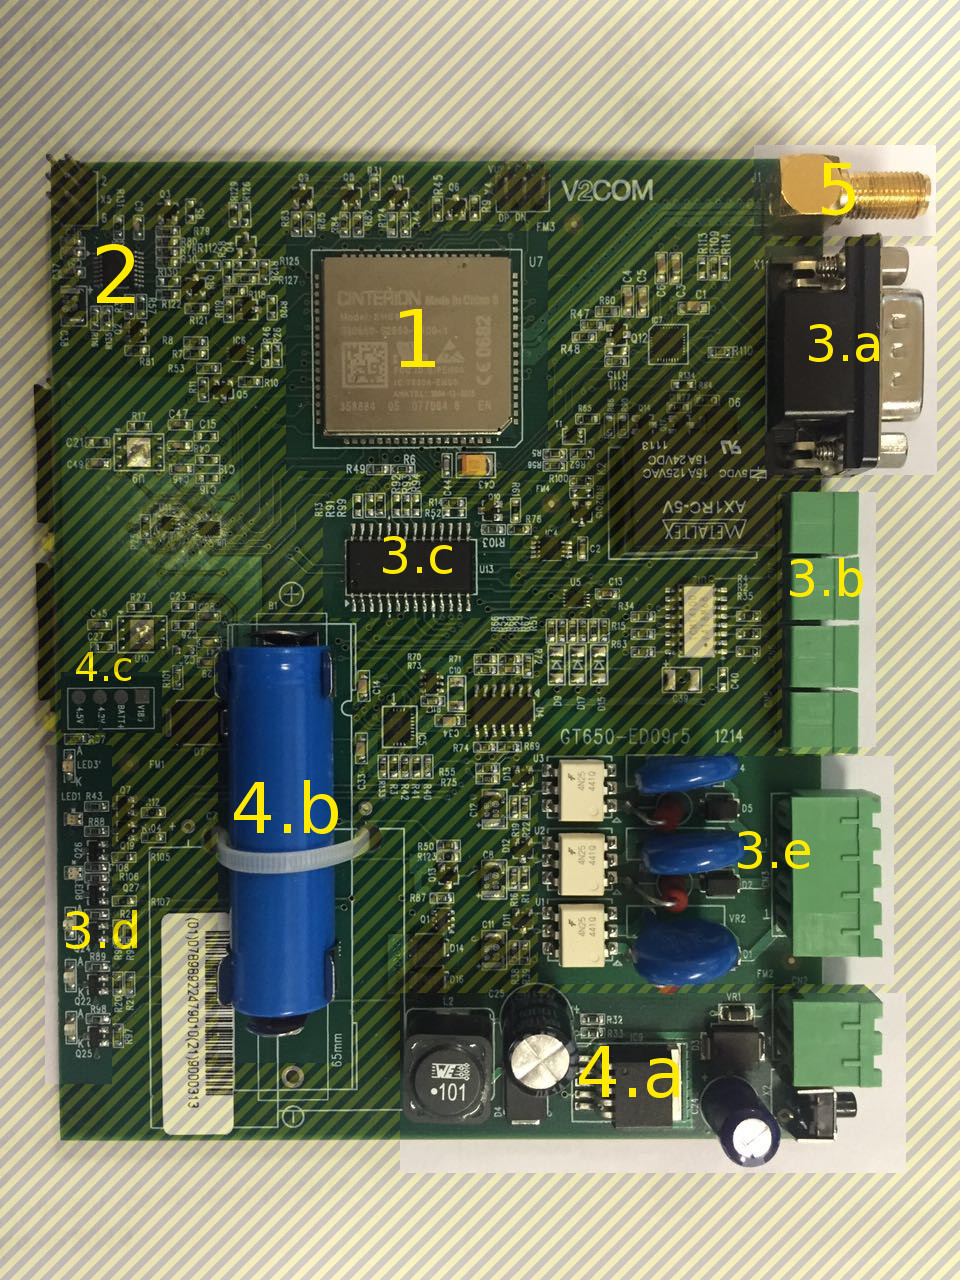
\includegraphics[width=0.92\linewidth]{placa}
        \caption{Foto do GT650 com destaque aos componentes da placa: o \textit{modem} EHS6 (1); o microcontrolador monitor \textit{watchdog} (2); o conector DB9 com duas portas RS232 (3.a); as E/S isoladas (3.b); o expansor de E/S por I$^{2}$C (3.c) ; o painel de LEDs indicativos (3.d); os detectores de tensão trifásica (3.e); o conversor buck (4.a); a bateria e o seu sistema de gerenciamento (4.b); os pontos de teste de alimentação (4.c); e o conector da antena (5) (foto do autor).}
        \label{fig:placa}
    \end{figure}
    
    \subsection{Módulo M2M}
        O \textit{modem} EHS6 da Cinterion (ponto 1 da figura \ref{fig:placa}) é o processador principal da placa, com comunicação TCP/IP via GSM/3GPP/GPRS, Intepretador Java e outros recursos comuns, como interface serial e I$^{2}$C. Segundo o \textit{datasheet} do fabricante \citep{cinterion2016}, o circuito integrado oferece: 
        %todo cite EHS6 DATASHEET
        
        \begin{itemize}
            \item Comunicação de dados 3G (HSPA): 800/850/900/1900/2100 MHz
            \item GPRS/EDGE Class 12: 850/900/1800/1900 MHz
            \item Suporte a Java™ ME\footnote{Java Micro Edition é  uma plataforma Java para sistemas embarcados} 3.2, com suporte a \textit{multithreading} e execução de múltiplas aplicações, além de 6 MB de memória RAM e 10 MB de memória Flash;  %todo cite JAVA ME
            \item Pilha de protocolos TCP/IP embarcada e acessível por comandos AT, incluindo conexão segura via TLS/SSL; serviços DNS e Ping; Cliente FTP e HTTP; %todo cite AT Commands
            \item Interface USB 2.0 HS e duas portas de interface modem serial;
            \item 16 GPIOs compartilhadas com as portas de comunicação, PWM e outras.
            \item ADC e interface I$^{2}$C; 
            \item Atualização de \textit{Firmware Over-the-air} (FOTA).
        \end{itemize}
        
        O fabricante não fornece informações internas sobre a arquitetura, como também nenhum meio de acesso à estrutura interna do módulo, como uma porta JTAG. Como contrapartida, a empresa oferece garantia de funcionamento, assim como suporte técnico completo. As consequências dessa política não são necessariamente positivas, conforme segue:
        
        Primeiro, impede a realização de testes estruturais e verificações mais profundas nos módulos, tanto na produção, quanto na manutenção, e torna todos os processos dependentes de agentes externos, de forma que o teste se limita à verificação de interconexões do \textit{modem} com seus periféricos, em um esquema similar aos testes centralizados por processador, vistos em \ref{FCT}. Outra dificuldade do EHS6 é seu encapsulamento LGA, que impede a completa verificação de solda por inspeção visual. Isso pode ser contornado, caso a empresa responsável pela montagem possua equipamentos de inspeção radiográfica.
        
        Segundo, que para todo e qualquer problema físico ou de \textit{firmware} que ocorrer com estes módulos, é necessário o envio ao fabricante original para solução, muitas vezes dependendo do suporte deste fornecedor em outro país. Por um lado, isto retira da empresa solicitante a responsabilidade de resolver problemas de baixo nível, assim como a necessidade de manter pessoal e equipamento especializado para analisar este tipo de falha. Por outro lado, trabalhar com componente e \textit{firmware} fechados deixa a produção sujeita a problemas invisíveis e cria uma situação de dependência com o OEM.
        
        Por estas limitações no teste estrutural, o escopo de teste elaborado é restrito às verificações funcionais administradas pelo próprio produto. 
        
    \subsection{Monitor \textit{Watchdog}}
    
        O MC9S08QG8 é um microcontrolador simples de 8 bits (figura \ref{fig:placa}, no ponto 2) e é  responsável por desligar o \textit{modem} por duas maneiras: a primeira pelo temporizador \textit{watchdog} e a segunda, pelo botão liga-desliga. 
        
        Também é armazenado nele o número de série da placa. Dessa forma, a empresa consegue separar o rastreamento dos \textit{modems} e das \emph{placas}, podendo intercambiá-las conforme necessário.
        
        Por estar conectado ao EHS6 como escravo I$^{2}$C, este componente é acessado e testado pelo mesmo. No teste funcional são realizadas as seguintes rotinas: captura do número de série, teste do botão liga-desliga e teste do temporizador \textit{watchdog}.
        
    \subsection{Interfaces de usuário e interconexões externas}
        Por ser uma solução de comunicação para outros equipamentos, o GT650 não possui interfaces digitais e analógicas muito complexas, exceto pela comunicação de dados via GSM, que será descrita à parte. Como pode ser visto na figura \ref{fig:placa}, a placa possui:
        
        \begin{itemize}
            \item Duas portas RS232\footnote{Uma é usada para comunicação por comandos AT e a outra para acessar os periféricos na porta I$^{2}$C};
            \item Três portas de entrada digitais opto isoladas; 
            \item Um relé de saída;
            \item Seis LEDs de sinalização;
            \item Uma porta para conferência de tensão trifásica.
        \end{itemize}
        
        Vale mencionar que as entradas e saídas digitais, assim como os LEDs, são controlados pelo \textit{modem} através do expansor de GPIO por endereçamento I$^{2}$C. Assim como no caso do microcontrolador de \textit{watchdog}, as verificações funcionais são acionadas pelo EHS6.

    \subsection{Conector e transmissor de radiofrequência (RF)}            
        
        O módulo não possui antena integrada e possui um conector SMA para a conexão de antenas externas. Neste caso, testa-se a potência do transmissor de radiofrequência através de um instrumento específico mencionado na seção \ref{instruni}.
            
    \subsection{Alimentação, bateria e BMS}
        O sistema de alimentação consiste em um conversor CC-CC de 12 Volts com saídas de 3,3 V e 5 V (figura \ref{fig:placa}-4.a) e uma bateria de lítio de 4,8 V, em caso de faltas na rede (figura \ref{fig:placa}-4.b). 
        
        Para testar este sistema, foram separados quatro pontos de teste na placa, como visto no ponto 4.c da figura \ref{fig:placa}: 5V, BATT+, 3V3, e 1.8V. Atualmente, o teste é realizado manualmente com o multímetro, ponto por ponto, mas enviando os dados de leitura pelas portas seriais do computador. 
                
\section{Cobertura e roteiro de teste}
        
    O roteiro de teste consiste numa verificação predominantemente funcional da placa do produto. Por não possuir um volume de produção que justifique a aquisição de um ICT, não possuir suporte ao IEEE 1149.1, como também por não conter nenhuma lógica programável no produto, o teste estrutural se limita às verificações realizadas na empresa de montagem, por verificações de solda e interconexões por AOI ou AXI. 
        
    Essa estratégia predominantemente funcional consegue atingir um bom controle de qualidade dos lotes, mas fracassa no diagnóstico de falhas e detecção de causas raiz. 

    A bateria de testes do produto é representada pelo fluxograma da figura \ref{fig:flowchart}. Nota-se que este roteiro é, em sua totalidade, sequencial, sendo o teste funcional das bandejas do cartão SIM a única etapa executada de forma concorrente. 
    
    \begin{figure}[h]
        \centering
        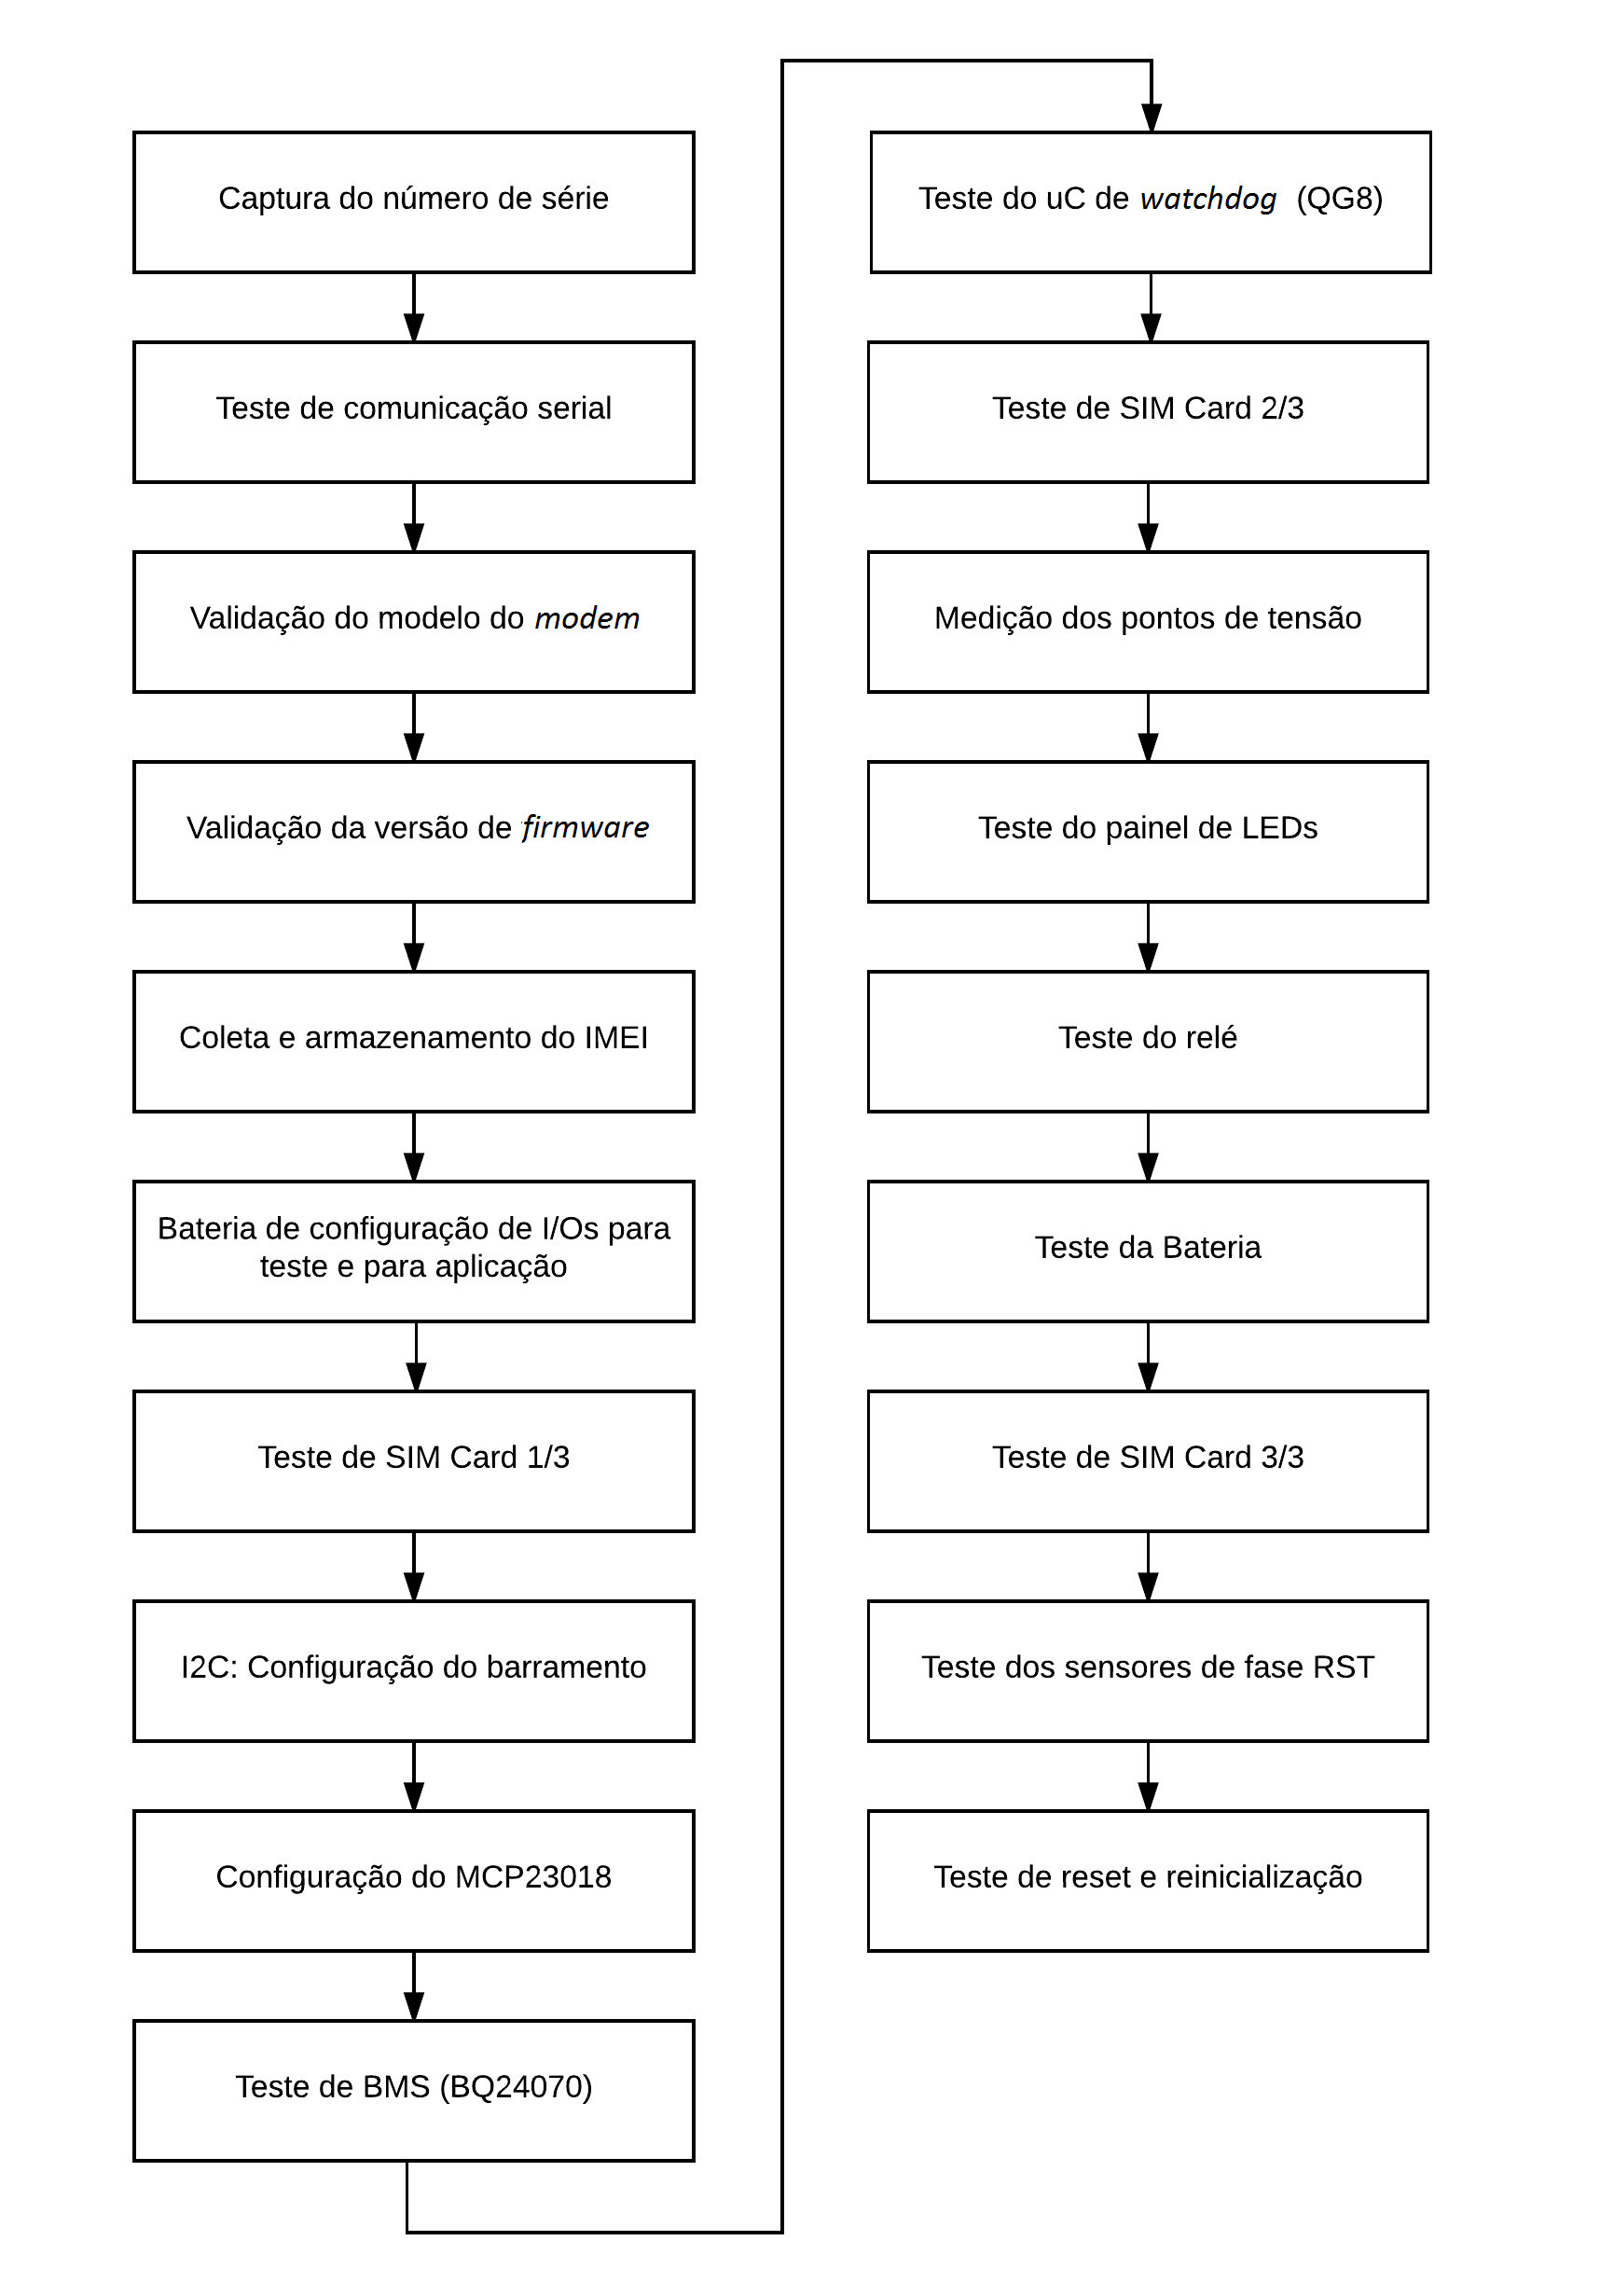
\includegraphics[width=0.9\textwidth]{model/fluxograma}
        \caption{Fluxograma da bateria de testes}
        \label{fig:flowchart}
    \end{figure} 
   
\section{A Jiga e os instrumentos de teste}
        
    A jiga utilizada foi desenvolvida para o teste funcional e provê interconexão para as interfaces externas do produto, exceto para o transmissor de radiofrequência. Fornece botões de interface para o operador controlar estímulos simples de sinais lógicos nas entradas e emular tensões trifásicas na porta respectiva. Ela também oferece um ponto de conexão do terra da placa para utilização do multímetro digital.
    
    \subsection{Multímetro}
        
        O multímetro utilizado é um ICEL MD-6400, com suporte de comunicação por uma porta serial RS232. A figura \ref{fig:dmmprotocol} exibe o protocolo que, a cada 250 ms, envia pacotes de 14 bytes de dados a uma \textit{baudrate} de 9600. 
          \begin{figure}[ht]
                \centering
                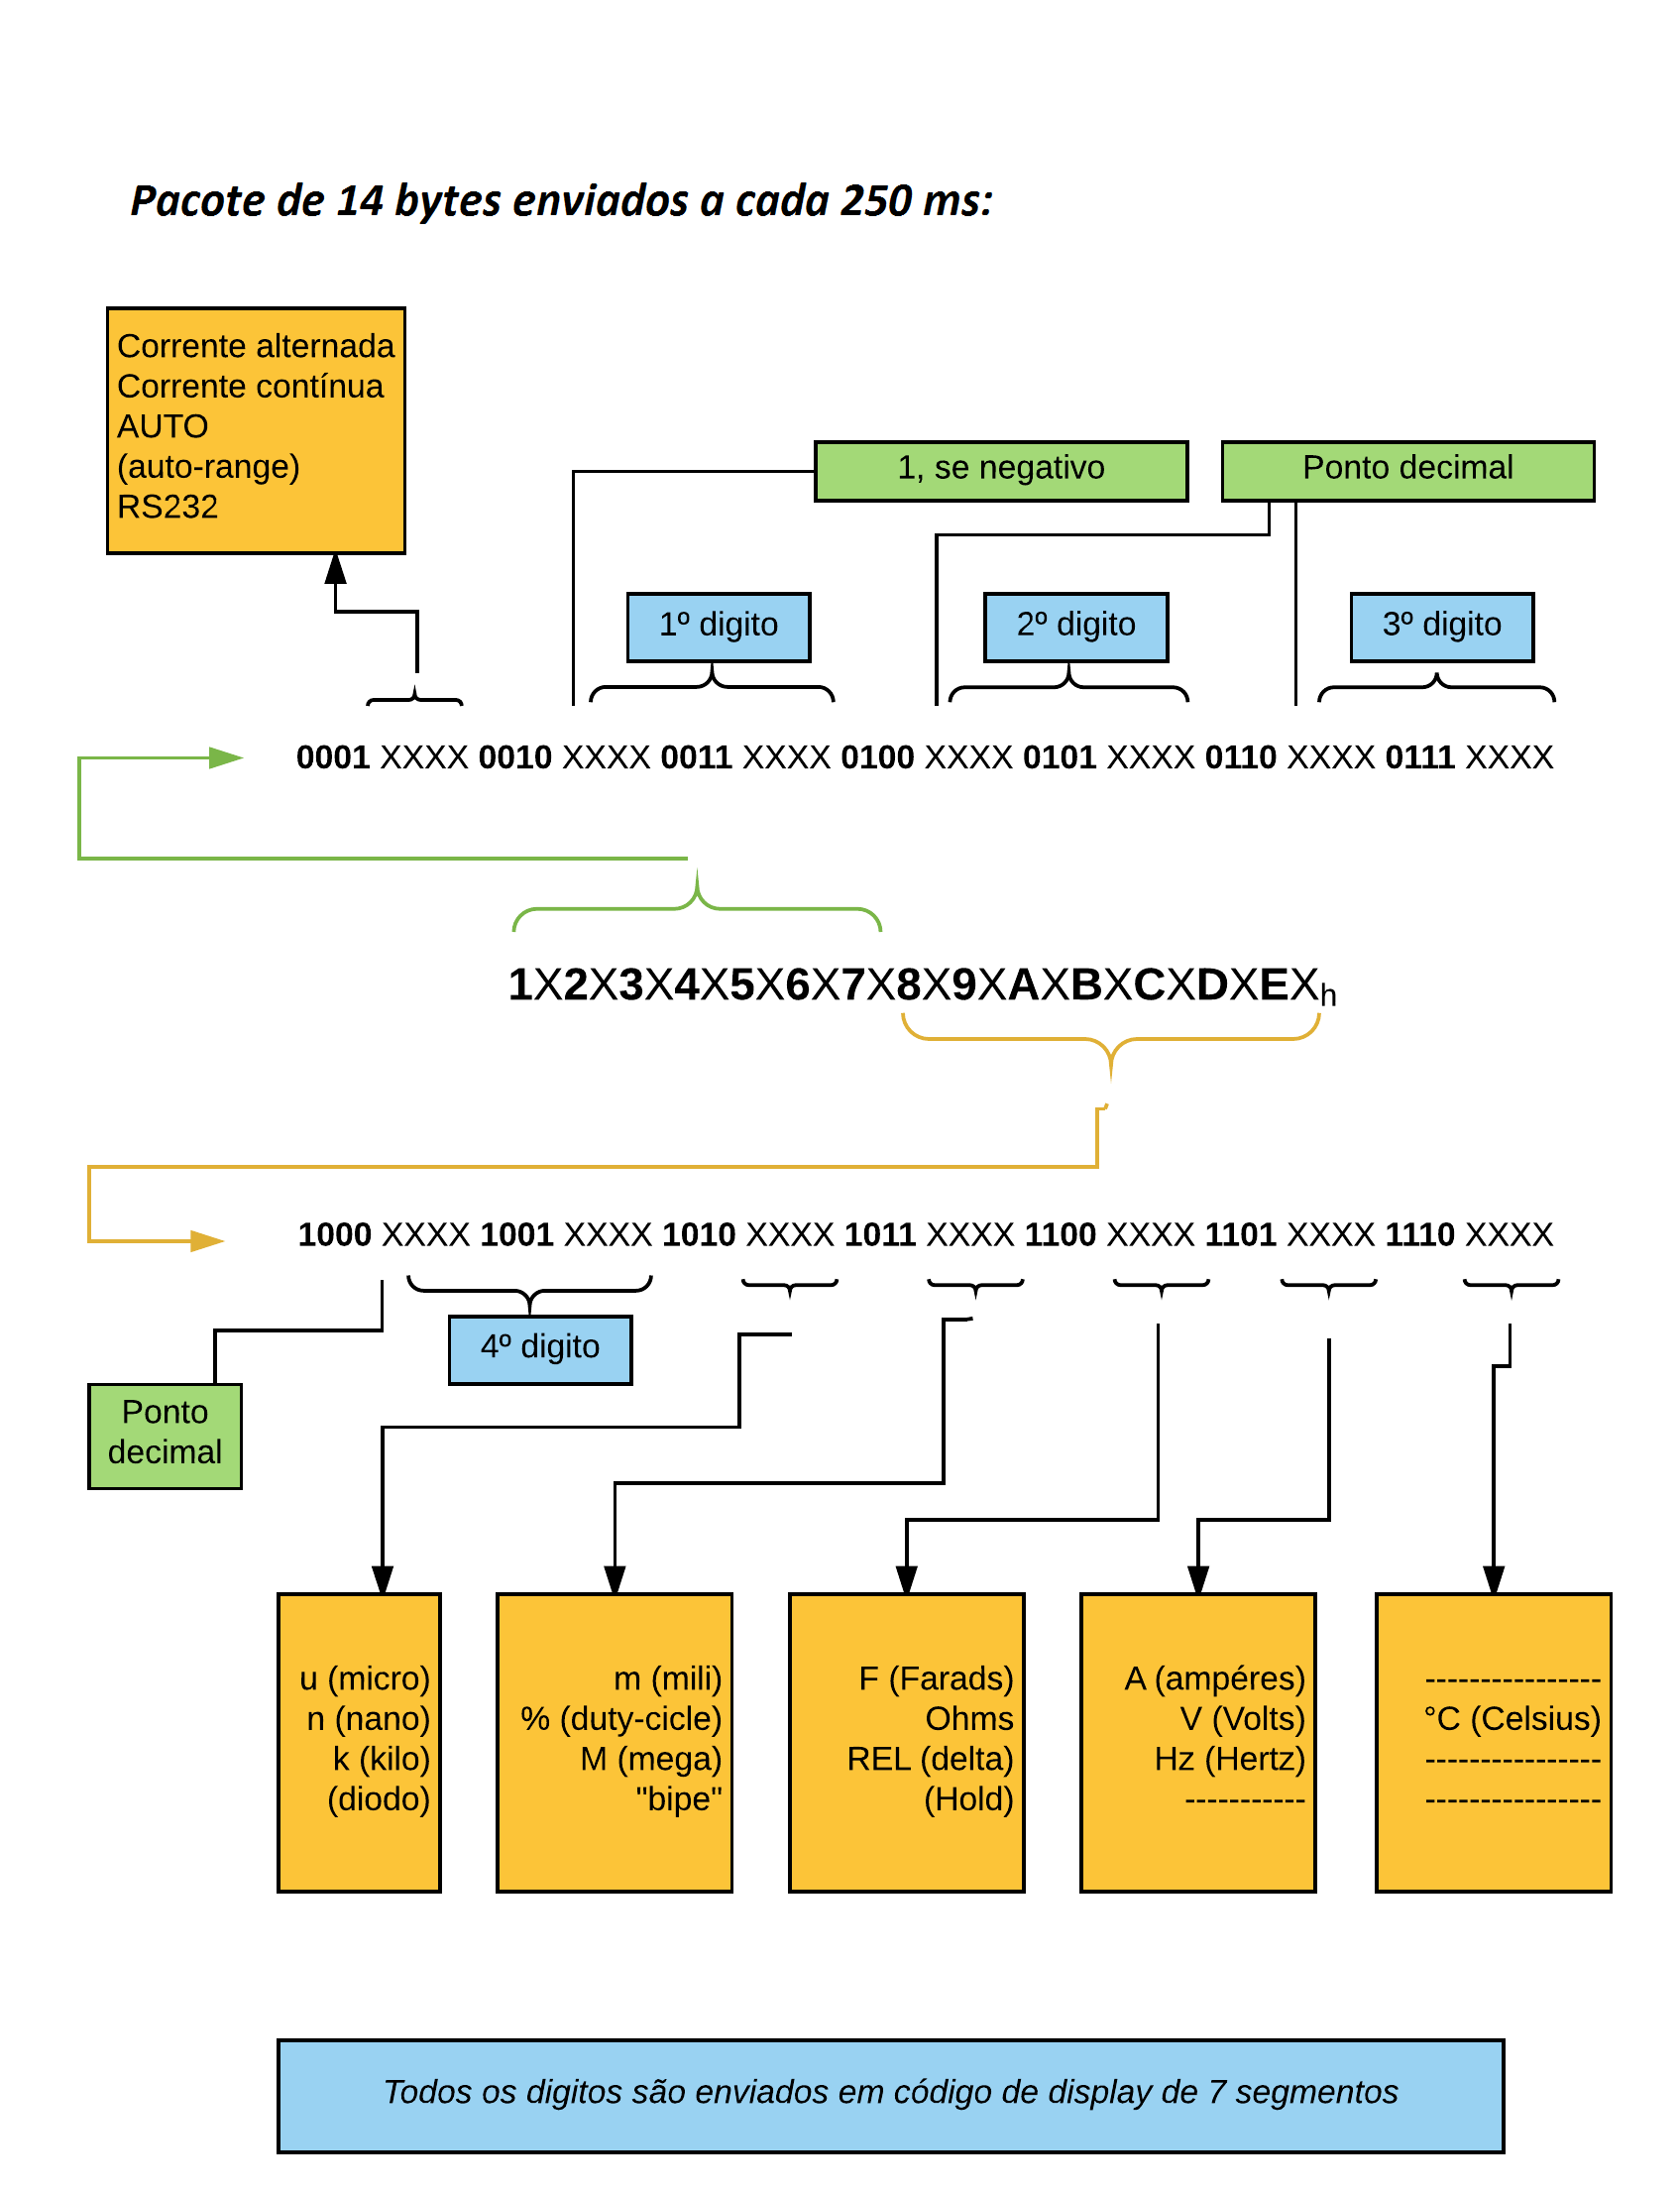
\includegraphics[width=\textwidth]{model/dmmprotocol}
                \caption{Estrutura de pacote de comunicação do multímetro}
                \label{fig:dmmprotocol}
            \end{figure}
    
    \subsection{Medidor de potência do transmissor}
    \label{instruni}
    % falar do programa de teste de potencia realizado anteriormente?
        O instrumento de medição de potência RF utilizado foi o NI 5680, da National Instruments, que mede potência RMS de sinais até 6 GHz, em larguras de banda bem estreitas (10-100 Hz de banda), e um limites de potência de entrada de -40 dBm a +23 dBm.

        \begin{figure}
            \centering
            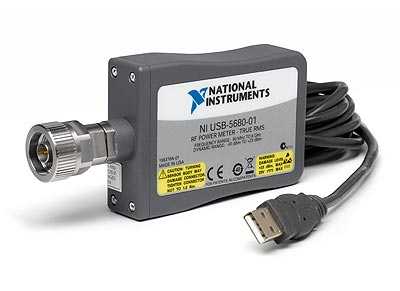
\includegraphics[width=0.7\textwidth]{usb5680.jpg}
            \caption{NI 5680 - instrumento utilizado para medição de potência RF}
            \label{fig:ni5680}
        \end{figure}
    
        % inserir http://sine.ni.com/nips/cds/view/p/lang/pt/nid/204499
        % datasheet http://www.ni.com/pdf/products/us/CAT_USB5680.pdf
        
        %falar como a bateria de medidas foi elaborada e a qualidade    delas
        
        % Atualmente é usado um medidor de potência RF -- O \emph{NI USB-5680} -- que tem uma faixa de frequência 50 MHz até 6 GHz, alcance de potência de -40 a +23 dBm, e uma banda de canal 10 a 100 MHz. Esta nova estratégia adotada, praticamente eliminou os retornos de campo por problemas de alcance do produto.
    
\section{Requisitos de Software}

        Requisitos de software são objetivos ou restrições estabelecidos pelos usuários e são divididos em requisitos funcionais e não funcionais \citep{bourque2014guide}.
        
        Requisitos funcionais definem as funcionalidades específicas que o programa deve oferecer, não necessariamente tratando das interações com o usuário, mas também como funcionalidades ocultas como, por exemplo, uma API ou interações com hardware.
        
        Requisitos não-funcionais são qualidades gerais de um programa como custo, usabilidade, modularidade e vários outros. Normalmente são requisitos difíceis de validar por sua natureza qualitativa. 
        
        A partir do contexto apresentado, foram levantados os seguintes requisitos não-funcionais do software:
        \begin{itemize}
            \item O programa deverá ser implementado em LabVIEW;
            \item Modularidade do programa e reusabilidade de código;
            \item Permitir o uso de concorrência e paralelismo na bateria de testes;
            \item Escalabilidade e flexibilidade de software para acompanhar alterações de hardware e da jiga de teste;
            \item Interface de usuário ergonômica e intuitiva.
        \end{itemize}
        
        Já os requisitos funcionais de software acompanham o que é testado pelo roteiro de testes anterior a este trabalho:
        \begin{itemize}
            \item Leitura e armazenamento do número de série colado na placa por um leitor de código de barras;
            \item Comunicação com o DUT via serial;
            \item Teste de comunicação das duas portas seriais;
            \item Verificação do modelo de \textit{modem};
            \item Verificação da versão da \textit{firmware} do \textit{modem};
            \item Armazenamento o IMEI\footnote{\textit{International Mobile Station Equipment Identity} ou Identificação Internacional de Equipamento Móvel é um número de identificação global e único para cada telefone ou \textit{modem} celular.} do \textit{modem};
            \item Configuração das GPIOs do \textit{modem} conforme o perfil da aplicação;
            \item Abertura, seleção e teste das duas bandejas de cartão SIM\footnote{\textit{Subscriber Identity Module}};
            \item Configuração e teste de comunicação $I^{2}C$;
            \item Configuração da operação do expansor de IO, MCP23018: interrupção espelhada, não incremento de ponteiro, interrupção push-pull;
            \item Configuração e teste do BQ24070, carregador de bateria e gerenciador de energia do sistema;
            \item Teste de leitura da bateria;
            \item Teste do MC9S08QG8, microcontrolador \textit{watchdog} e teste do botão liga e desliga;
            \item Leitura do número de série armazenado no MC9S08QG8, e validação deste com o número de série colado na placa;
            \item Teste de comunicação e leitura do sensor de temperatura LM75;
            \item Teste de finalização da sessão do terminal na porta serial ;
            \item Testes dos barramentos de tensão da placa: 4,5V, 4,2V, BATT++ e 1,8V;
            \item Teste do painel de LEDs;
            \item Teste de detecção de retirada e inserção da fonte de alimentação;
            \item Teste das 3 portas digitais;
            \item Teste de acionamento e desarme de relé;
            \item Teste da porta de tensão trifásica - detecção de presença e ausência;
            \item Teste de interrupção de desligamento e reinicialização do sistema;
            \item Teste de potência de sinal do transmissor de radiofrequência;
            \item Registro de execução de teste em arquivo de texto e resumo de teste em formato estruturado;
            \item Cliente WEB para envio automático à base de dados de produtos;
            \item Notificação para o operador sobre sucesso ou falha do teste, assim como possibilidade de reteste.
        \end{itemize}
    
    
    %Registro em servidor

    %A segunda classe de registro é um resumo estruturado da bateria de testes, o diagnóstico geral da placa e outras informações importantes para o controle e rastreamento dos produtos, requisito necessário para otimizações do processo produtivo como também do próprio produto.

\begin{comment}
    \subsection{Workflow do projeto} % jeitinho de trabalhar
       
     
     %   \subsection{Síntese dos requisitos ambientais de teste}
    % #todo
    
    Validação do projeto
    Controle de Qualidade
    Melhorias de processos
    Melhorias no produto
    Auxilio na Manutenção
\end{comment}    